\documentclass[12pt, a4paper, oneside]{article}
\usepackage[english]{babel}
\usepackage{xcolor,listings}
\usepackage{hyperref}
\usepackage{mathtools}
\usepackage{amsmath}
\usepackage{datetime}
\usepackage{graphicx}
% For fitting table to page
\usepackage{adjustbox}
% For pseudocode
\usepackage{algorithm}
% Ensure section stays in place when adding images
\usepackage[section]{placeins}
\usepackage[noend]{algpseudocode}
\makeatletter
\def\BState{\State\hskip-\ALG@thistlm}
\makeatother
%

\setlength{\parindent}{0pt}

\begin{document}
\title{ECE 495/595: Speech Analysis Initial Requirements Document}
\author{
  Grace, Jayson \\
  \texttt{jaysong@unm.edu}
  \and
  Rutherford, Amber \\
  \texttt{anhruthe@gmail.com}  
  \and
  Sampelli, Meghana \\
  \texttt{meghana.sampelli2811@gmail.com}
  \and
  Kim, Nicole \\
  \texttt{nkim0912@salud.unm.edu}
  \and
  Gordon, Jeffrey \\
  \texttt{jeffreyrgordon@gmail.com}
  \and
  Dara, Harish \\
  \texttt{harish225@unm.edu} 
}
\date{\today}%
\maketitle

\pagenumbering{gobble} 
\pagebreak
\pagenumbering{arabic}

\section*{Problem Statement}
Our team will create an application that enables a user to associate a speaker with the phonemes they spoke when reading through a prescribed paragraph. These speakers will in turn be associated with users that manually input the phoneme information as it corresponds to letters or clusters of letters. \\

Once data has been entered, our client will be able to run relevant queries on the input data to enumerate relationships that are useful for her research. These queries will appear in drop down menu combinations due to the way that ActiveRecord abstracts away the SQL component of interfacing with databases. The users will also be able to view the information they’ve input in order to ensure that it is error-free and consistent.

\section*{Client Requirements}
\begin{enumerate}
\item The application must have a Login/Sign up page for users.

\item Overview page when viewed as the client will have options to create a speaker, enter phonemes for a speaker and the ability to view and query view all existing phoneme data.

\item Overview page for students will only show the options to enter phonemes for a speaker and view the speaker data that they have entered previously.

\item The speaker speech input page will display a paragraph that each student or the client will use as a point of reference for entering speech data.

\item Speaker speech page must have references to help the students and client interpret the phoneme with specific speech accents.

\item Each word will have two text boxes to be filled out, one for the phonemes from the referenced text file and the other for base phonemes.

\item All input fields for a speaker to enter phonemes must be filled out before information can be submitted. 

\item There should be the same number of commas for both of the input fields.

\item Validations will be present to ensure that the fields for all of the words are present before the user attempts to submit any data. 

\item After all of the data has been submitted, the client will be able to view all data associated with the speaker that they’ve input.

\item The client will be able to view all speaker data that any user has input.

\item Three tables will created be used to encompass authorization, speaker information and phoneme information.

\item There will be a link that documents how to correctly fill out the input fields.
\end{enumerate}

\section*{Scope}
Our client Amy Neel, Associate Professor, Dept. of Speech and Hearing Sciences, has requested the creation of this project to develop and assist the department in meeting its research goals. This will increase the department’s knowledge of the data pertaining to phonemes and speakers from different ethnic backgrounds. Upon completion, this project will provide an interface to populate a large dataset that can be used for future research in this area. \\

\subsection*{Project Product}
\begin{enumerate}
\item \textbf{Tools:} The website will allow users to input phonemes of speech patterns across varying ethnicities, and view all of their completed input. The database will store that data in a safe environment, for purposes of reference and retrieval. 
 
\item \textbf{Users:} Users will consist of students that are assigned one or more speaker(s), and given the task of completing phoneme translations for that speaker.

\item \textbf{Client:} The client, who is not considered a user, will have access to phoneme exercises, view all user data, query data, and enter speaker information. 
\item \textbf{Exercises:} Exercises will consist of an image that displays the phoneme, a set of text that each speaker has read, an entry box for phonemes, and an entry box for mapping those phonemes to a static list of numbers from 1 to 255. Each word in the sentence will contain one box per phoneme entry, and one box for mapping. All entry boxes in the exercise must be completed and submitted in order for the exercise to be considered complete. If a speaker has omitted an entire word, there would still be commas to represent the lack of data. Commas will be used in each box as a means for identifying all required entries whether they are phonemes, blanks, or mapping numbers.

\item \textbf{Query:} The client will be able to query the data within the database which includes entry information, speaker information, and user information.
\end{enumerate}

\subsection*{Project Deliverables}
Gantt chart, requirements document, scope, wireframes, system overview, final presentation, entity-relationship diagram (ERD), database backend, client user interface, and any other document related to the project. 
\begin{enumerate}
\item \textbf{Website:} A website will be developed for the department of Speech and Hearing Sciences. The website will include a user authorization page, a main page for navigating the site, a “Create Speaker” page, a “Speaker Entry” page, a “View Input” page, and a “Query” page. The only pages viewable to the user will be the Speaker Entry page, and the View Input page.

\item \textbf{Database:} A database will be developed that will contain a table for speakers and associate these speakers with phonemes. It will also contain a table of users that will be associated with speakers. The three tables included in the database are Authorization, Speakers, and Phonemes.
\end{enumerate}

\subsection*{Project Non-Deliverables}
In order to deliver this project in a timely and quality manner, any additional requirements or features which have not been described within this document will not be designed or developed as part of this project. 

\subsection*{Project Objective}
Create a database for storing all data regarding the phoneme exercises given by the department of Speech and Hearing Sciences. Create a user interface for users to complete phoneme exercises and for the client to view, and query the data resulting from user input.

\pagebreak 

\section*{Wireframe Images}
We have included some wireframe images to get some perspective on what the application could look like.

\begin{figure}
\centering
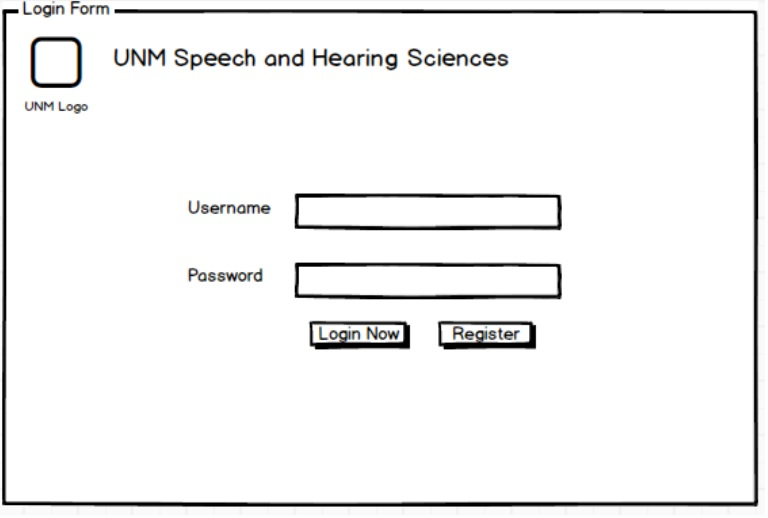
\includegraphics[width=\textwidth,height=\textheight,keepaspectratio]{./images/Wireframes/Login.jpg}
\caption{Login Page}
\end{figure}

\begin{figure}
\centering
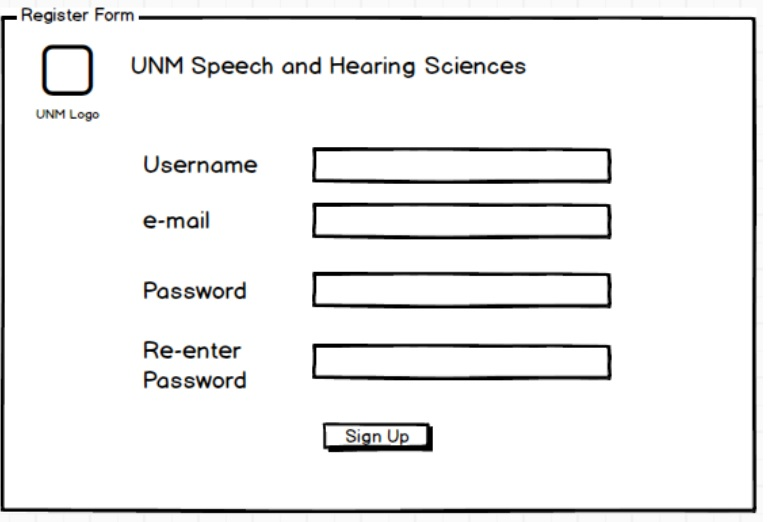
\includegraphics[width=\textwidth,height=\textheight,keepaspectratio]{./images/Wireframes/Register.jpg}
\caption{Registration Page}
\end{figure}

\begin{figure}
\centering
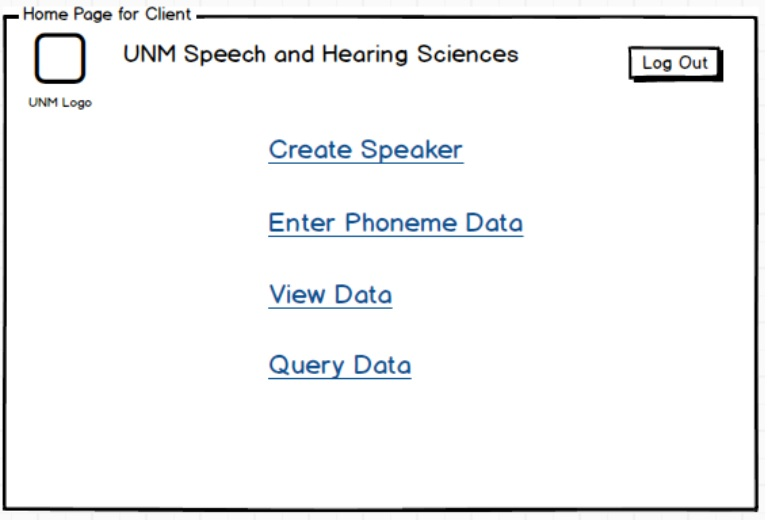
\includegraphics[width=\textwidth,height=\textheight,keepaspectratio]{./images/Wireframes/Homepage.jpg}
\caption{Homepage for Client}
\end{figure}


\begin{figure}
\centering
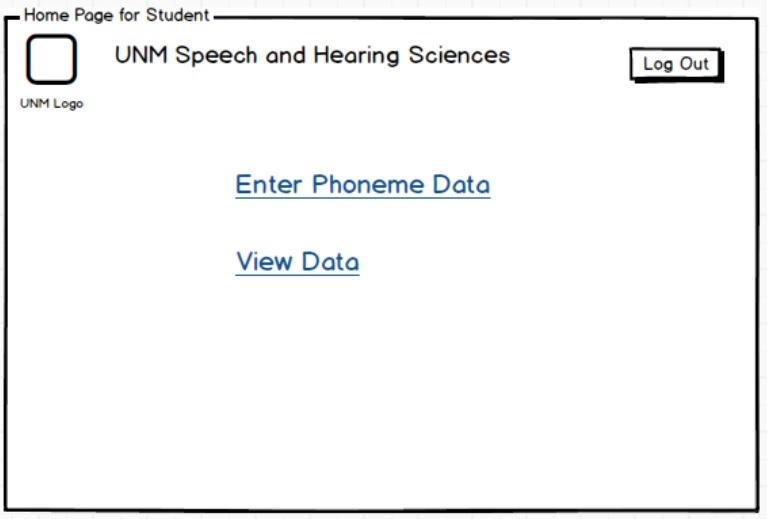
\includegraphics[width=\textwidth,height=\textheight,keepaspectratio]{./images/Wireframes/Homepage1.jpg}
\caption{Homepage for User}
\end{figure}


\begin{figure}
\centering
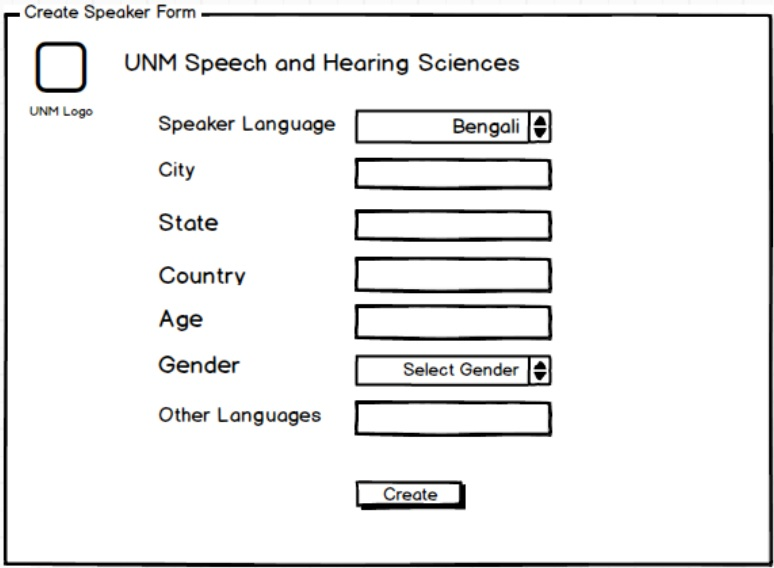
\includegraphics[width=\textwidth,height=\textheight,keepaspectratio]{./images/Wireframes/CreateSpeaker.jpg}
\caption{Speaker Creation Form}
\end{figure}


\begin{figure}
\centering
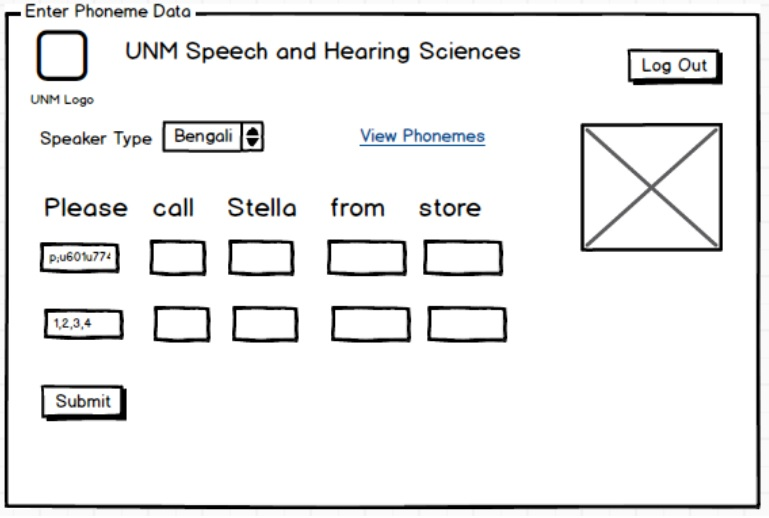
\includegraphics[width=\textwidth,height=\textheight,keepaspectratio]{./images/Wireframes/EnterPhoneme.jpg}
\caption{Phoneme Data Input Page}
\end{figure}


\begin{figure}
\centering
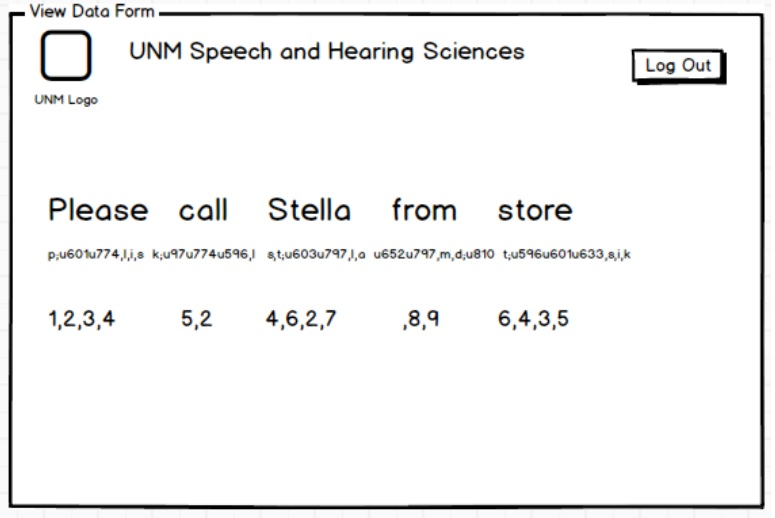
\includegraphics[width=\textwidth,height=\textheight,keepaspectratio]{./images/Wireframes/ViewData.jpg}
\caption{Data View}
\end{figure}


\pagebreak 
\section*{Gantt Chart}
The Gantt Chart outlines the timeline for work to be completed.

\begin{figure}
\centering
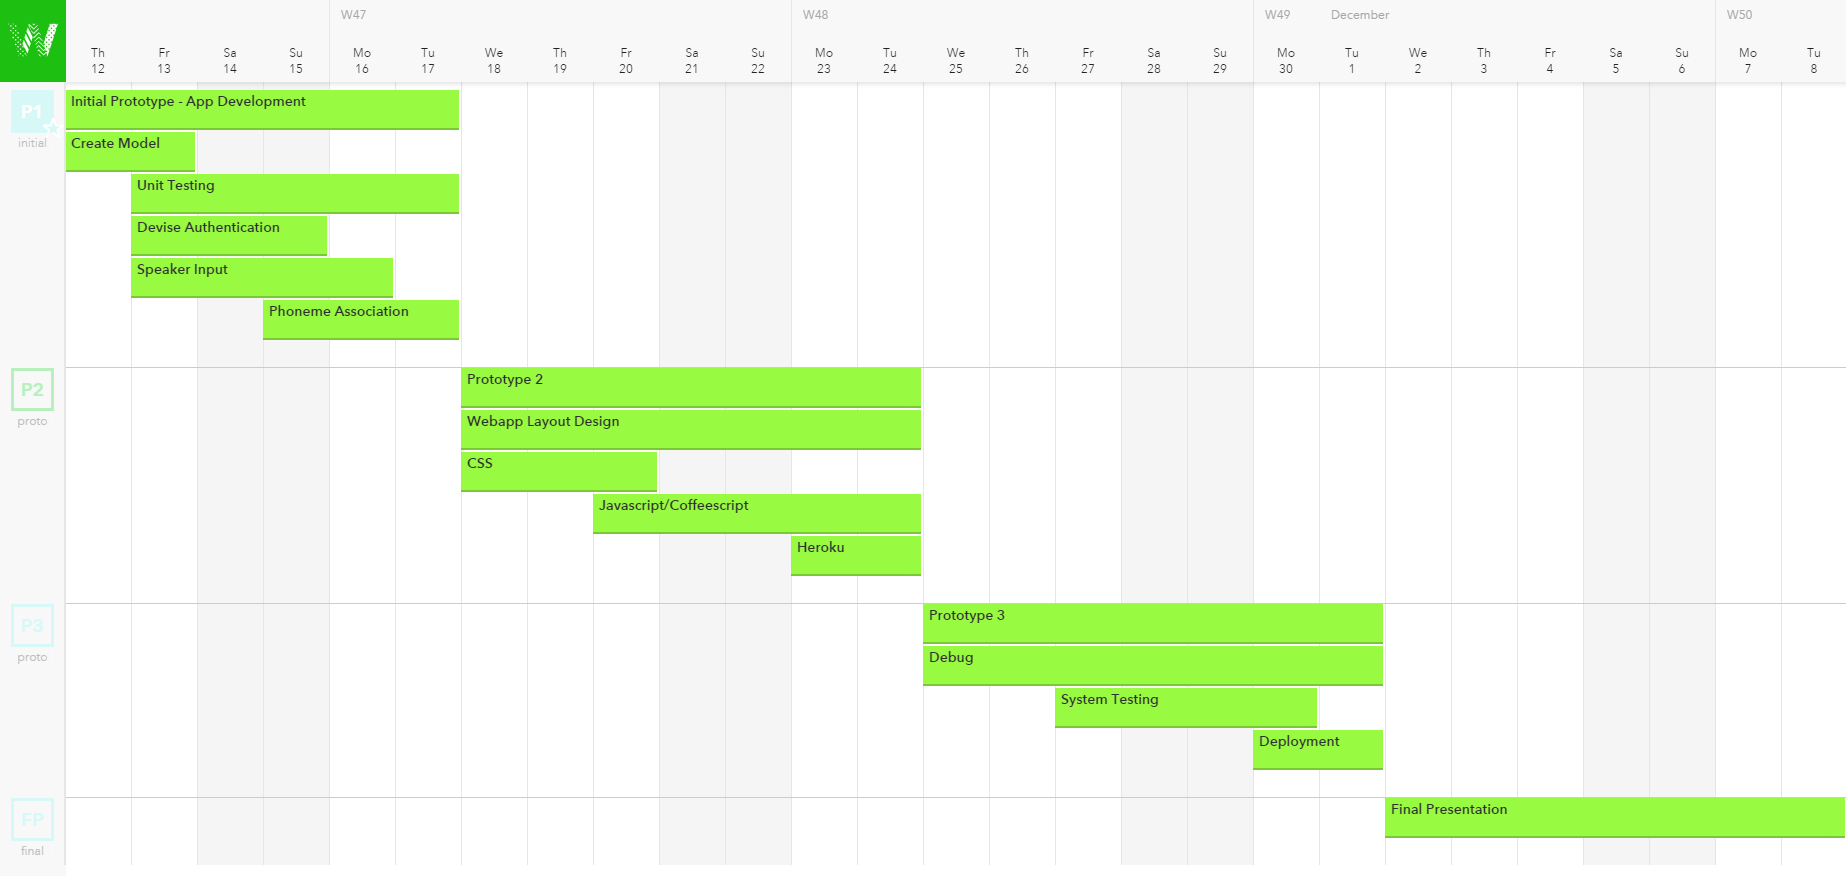
\includegraphics[width=\textwidth,height=\textheight,keepaspectratio]{./images/ganttchart.png}
\caption{Gantt Chart}
\end{figure}

\end{document}